\appendix

\section{Experiment 1 Methods}
\subsection{Definitions of the Nine Societal Causes}~\label{cause_def}

To ensure that the nine societal causes covered a broad spectrum of categories, we derived them from the categorization of charity groups on Amazon Smile, a popular donation website that has accumulated over 100 million dollars of donations. The categories were defined as:
\begin{enumerate}[label={},leftmargin=\parindent]
    \item (1) Pets and Animals: Animal Rights, Welfare, and Services; Wildlife Conservation; Zoos and Aquariums
    \item (2) Arts, Culture, Humanities: Libraries, Historical Societies, and Landmark Preservation; Museums; Performing Arts; Public Broadcasting and Media
    \item (3) Education: Early Childhood Programs and Services; Youth Education Programs and Services; Adult Education Programs and Services; Special Education; Education Policy and Reform; Scholarship and Financial Support
    \item (4) Environment: Environmental Protection and Conservation; Botanical Gardens, Parks and Nature Centers
    \item (5) Health: Diseases, Disorders, and Disciplines; Patient and Family Support; Treatment and Prevention Services; Medical Research
    \item (6) Human Services: Children's and Family Services; Youth Development, Shelter, and Crisis Services; Food Banks, Food Pantries, and Food Distribution; Multipurpose Human Service Organizations; Homeless Services; Social Services
    \item (7) International: Development and Relief Services; International Peace, Security, and Affairs; Humanitarian Relief Supplies
    \item (8) Faith and Spiritual: Religious Activities; Religious Media and Broadcasting
    \item (9) Veteran: Wounded Troops Services, Military Social Services, Military Family Support
\end{enumerate}

The participants saw the same definitions as shown above in the surveys during the study.

\section{Experiment 1 Results}

\subsection{Total Donation Amount}~\label{total_donation}
Figure \ref{fig:total_don_exp1} demonstrates two clusters for the total donation amount. 
The first cluster centered around $\$9-12$ with the majority in the range of $\$5$ to $\$20$. This group of people, making up about $60\%$ of the entire sample, donated part of the lottery winning amount but still kept a significant portion for themselves. The other clustered around $\$33$ to $\$35$, suggesting that this group of participants
contributed almost the full amount of the lottery prize. There were approximately $25\%$ of the participants who behaved this way. The total donation amount distribution across four surveying methods were relatively consistent, except that almost twice the proportion of participants in the Likert condition donated almost the full amount compared to the other QV conditions. One possible explanation for the difference is 
the Likert group required less effort compared to that of QV, and participants felt less tempted to earn an extra reward for their time spent in the Likert condition. 


\begin{figure}[htpb]
    \centering
    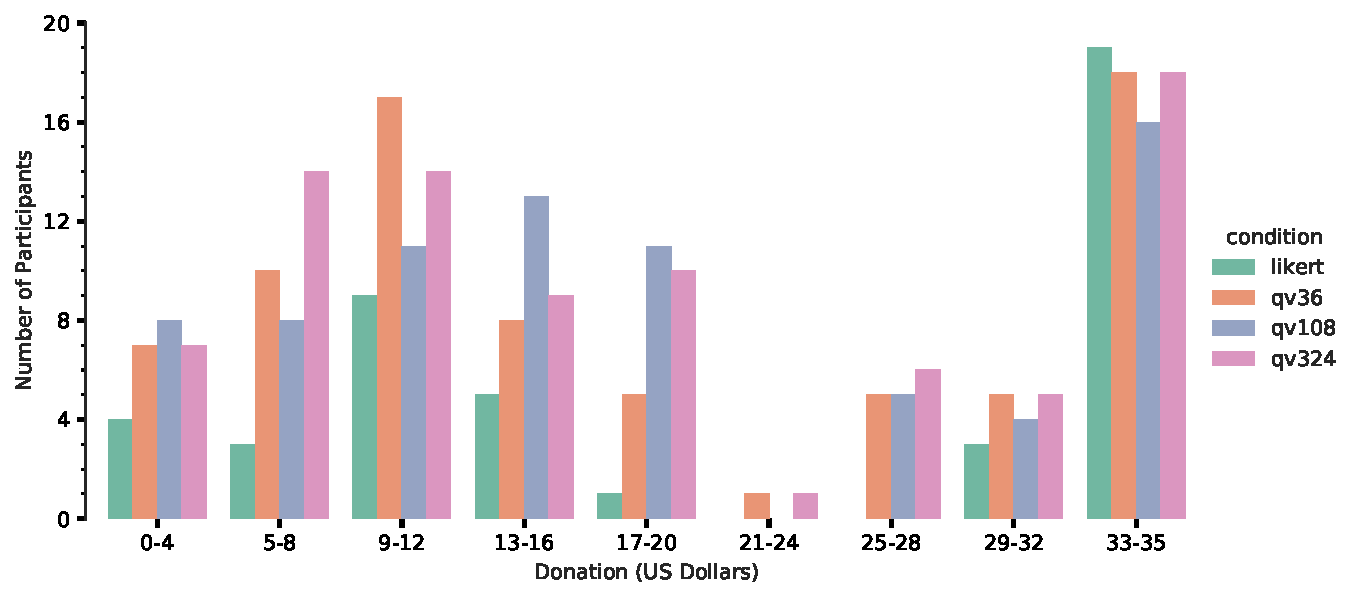
\includegraphics[width=\textwidth, keepaspectratio=true]{content/image/total_contributions_across_conditions.pdf}
    \caption{
       Distributions of the total amount donated by participants across four surveying methods.
       We see two distributions, one centered by $\$9-12$ and the other centered by $\$33$ to $\$35$.
       We also see more Likert participants donate almost most of their donation quota compared to the QV Groups.
    }
    \Description[Distributions of Total Donation Amounts across Groups for experiment 1]{ Distributions of the total amount donated by participants across four surveying methods.
    We see two distributions, one centered by $\$9-12$ and the other centered by $\$33$ to $\$35$.
    We also see more Likert participants donate almost most of their donation quota compared to the QV Groups.}
    \label{fig:total_don_exp1}
\end{figure}

\subsection{QV Budget Usage}
\begin{figure}[htpb]
    \centering
    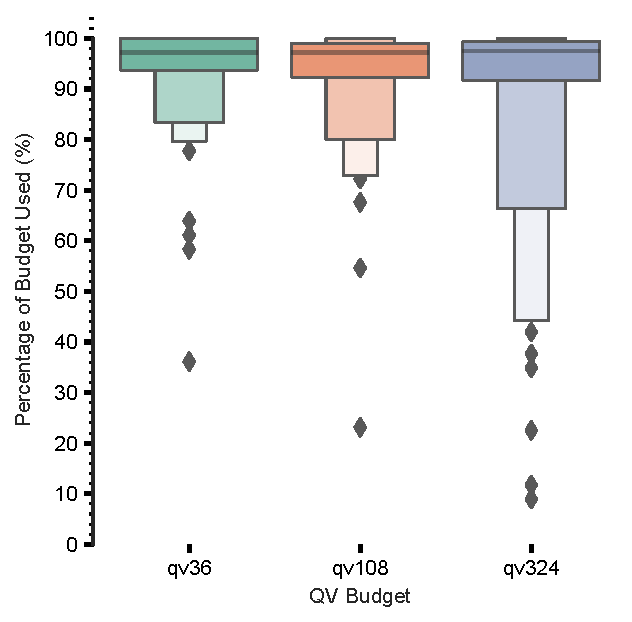
\includegraphics[width=0.5\textwidth, keepaspectratio=true]{content/image/qv_budget_used_distribution.pdf}
    \caption{
      Distribution of Percentage Budget Used in QV36, QV108 and QV324. Percentage budget used is the percentage of voice credits used out of the total voice credits budget available.
    }
    \Description[Distribution of Percentage Budget Used for experiment 1]{Distribution of Percentage Budget Used for experiment 1}
    \label{fig:qv_budget_exp1}
\end{figure}

\subsection{Posterior Predictive Check}
TO-DO

\subsection{Part Two}

Etiam commodo feugiat nisl pulvinar pellentesque. Etiam auctor sodales
ligula, non varius nibh pulvinar semper. Suspendisse nec lectus non
ipsum convallis congue hendrerit vitae sapien. Donec at laoreet
eros. Vivamus non purus placerat, scelerisque diam eu, cursus
ante. Etiam aliquam tortor auctor efficitur mattis.

\section{Online Resources}

Nam id fermentum dui. Suspendisse sagittis tortor a nulla mollis, in
pulvinar ex pretium. Sed interdum orci quis metus euismod, et sagittis
enim maximus. Vestibulum gravida massa ut felis suscipit
congue. Quisque mattis elit a risus ultrices commodo venenatis eget
dui. Etiam sagittis eleifend elementum.

Nam interdum magna at lectus dignissim, ac dignissim lorem
rhoncus. Maecenas eu arcu ac neque placerat aliquam. Nunc pulvinar
massa et mattis lacinia.